\chapauth{brylcreem}
\chapter{The Creature / Dying}


\section*{The creature. From the sewers.}

This wasn't going to happen. Again. Gene Beaver pulled off his light
suede jacket and sighed. Then he sighed again. He had started as a
trainee sewer inspector three months ago and immediately heard the
rumors. Rumors of a creature in the sewers.

Three years ago he had been happy. With a kid and another on the
way. Wife at home, making dinner. The whole nine yards. Then he came to
town. The kid. The prodigy they called him. Gene hated him. Hated him
enough to kill him? Perhaps. Or perhaps not. Either way, Gene hated him.

Two and half months later, his wife left him. With the kid. The kid from
out of town. Gene hated him, but he couldn't do anything about it.

It was Christmas, but Gene didn't feel jolly. Didn't feel jolly at
all. His wife was gone with the kids, and the kid and Gene was
alone. Alone at Christmas. The worst time of year to be alone. It was
sad. Suddenly, Gene sobbed.

No, this isn't right! He thought. Gene decided to change his life, to
make it better. A new life, in a new town.

Three years later, here he was. In the sewer, with a creature that
didn't show up.

Suddenly, Gene heard a sound. A sound from behind! Suddenly he turned
and came face to face with it! The creature! The rumors were real! The
creature was real!

Gene died quickly. In the sewers.

200 miles away, Louise shuddered in her sleep. The man next to her woke
and looked at her. And smiled!

\section*{Dying. Of arsenik!}



``Mommy? Where's Daddy?'' The questions kept
penetrating Louise's skull like a rusty icepick that had been
left outside too long. Long enough to develop rust. Cancer for
metal, Louise's father had always said in his father-voice. Now he
was dead. Like Gene.



``Daddy isn't here, sweetheart! We live with Tolkien now, remember?''
Louise had left Gene for Tolkien three years ago. It had been the
best years of her life. Until now. The kids made it that way. The
kids with their kid questions and their kid faces. Why were they
like that? They were kids, that's why.



Louise turned around. Suddenly! The kid winced. Louise slapped it
with her hand. Blood poured out of the mark left by her wedding
ring. Tolkien had bought it. On a Sunday.



They had visited Tolkien's parents. They lived in a small farmhouse
just off Route 66 in the desert. Miles to the neares neighbor. They
had horses, and Louise loved to ride them. Tolkien's parents were
rich. But it didn't show in the way they dressed. Tolkien's dad
wore shirts and blue jeans. Tolkien's mom wore shirts and blue
jeans. Tolkien had picked up the habit. He wore shirts and blue
jeans too. Soon, Louise were wearing shirts and blue jeans.



It was Sunday. Louise and Tolkien rode to town on a mighty steed.
They stopped at a jewellery store. Tolkien and Louise went inside
the jewellery store. Inside, the owner of the jewellery store
looked them up and down. She was the owner of the jewellery store,
and she didn't like poor people in her jewellery store, of which
she was the owner.



``Get out of my jewellery store!'' She said. ``We don't like poor
people in this jewellery store! I own this jewellery store!'' The
owner said.



``I have money!'' Tolkien said. He showed his money.



``Oh.'' The owner of the jewellery store said. ``Oh. Please shop. This
is my jewellery store''.



``Thank you.'' Tolkien said. ``I will'' he said.



Tolkien picked out a ring. He gave the money to the owner of the
jewellery store.



``Keep the change'' Tolkien said to the owner of the jewellery
store.



``Thank you very much'' the owner of the jewellery store said. Now
she could retire and buy a boat. Tolkien had been the 10.000th
customer and she had enough money to buy a boat and retire. So she
did, the next day.



In the meantime, Louise was happy with Tolkien. Tolkien wore shirts
and blue jeans. Louise wore shirts and blue jeans. The kids wore
pajamas. This was why Louise hated them.



She had been giving them arsenik for dinner every night. Her high
school biology teacher had taught her to make it in exchange for
sex. Louise had been 14 years old and she loved it. So did the
teacher. Louise told everything to the principal and he was fired.
Then he commited suicide. Louise didn't care.



Louise gave arsenik to her children. But what she didn't know, was
that the kids vomited from it. They vomited into the air ducts of
the house. And there the dust became infested with arsenik. Then
Louise and Tolkien breathed it and then they died.



The End. 
 




\begin{figure}[b]
  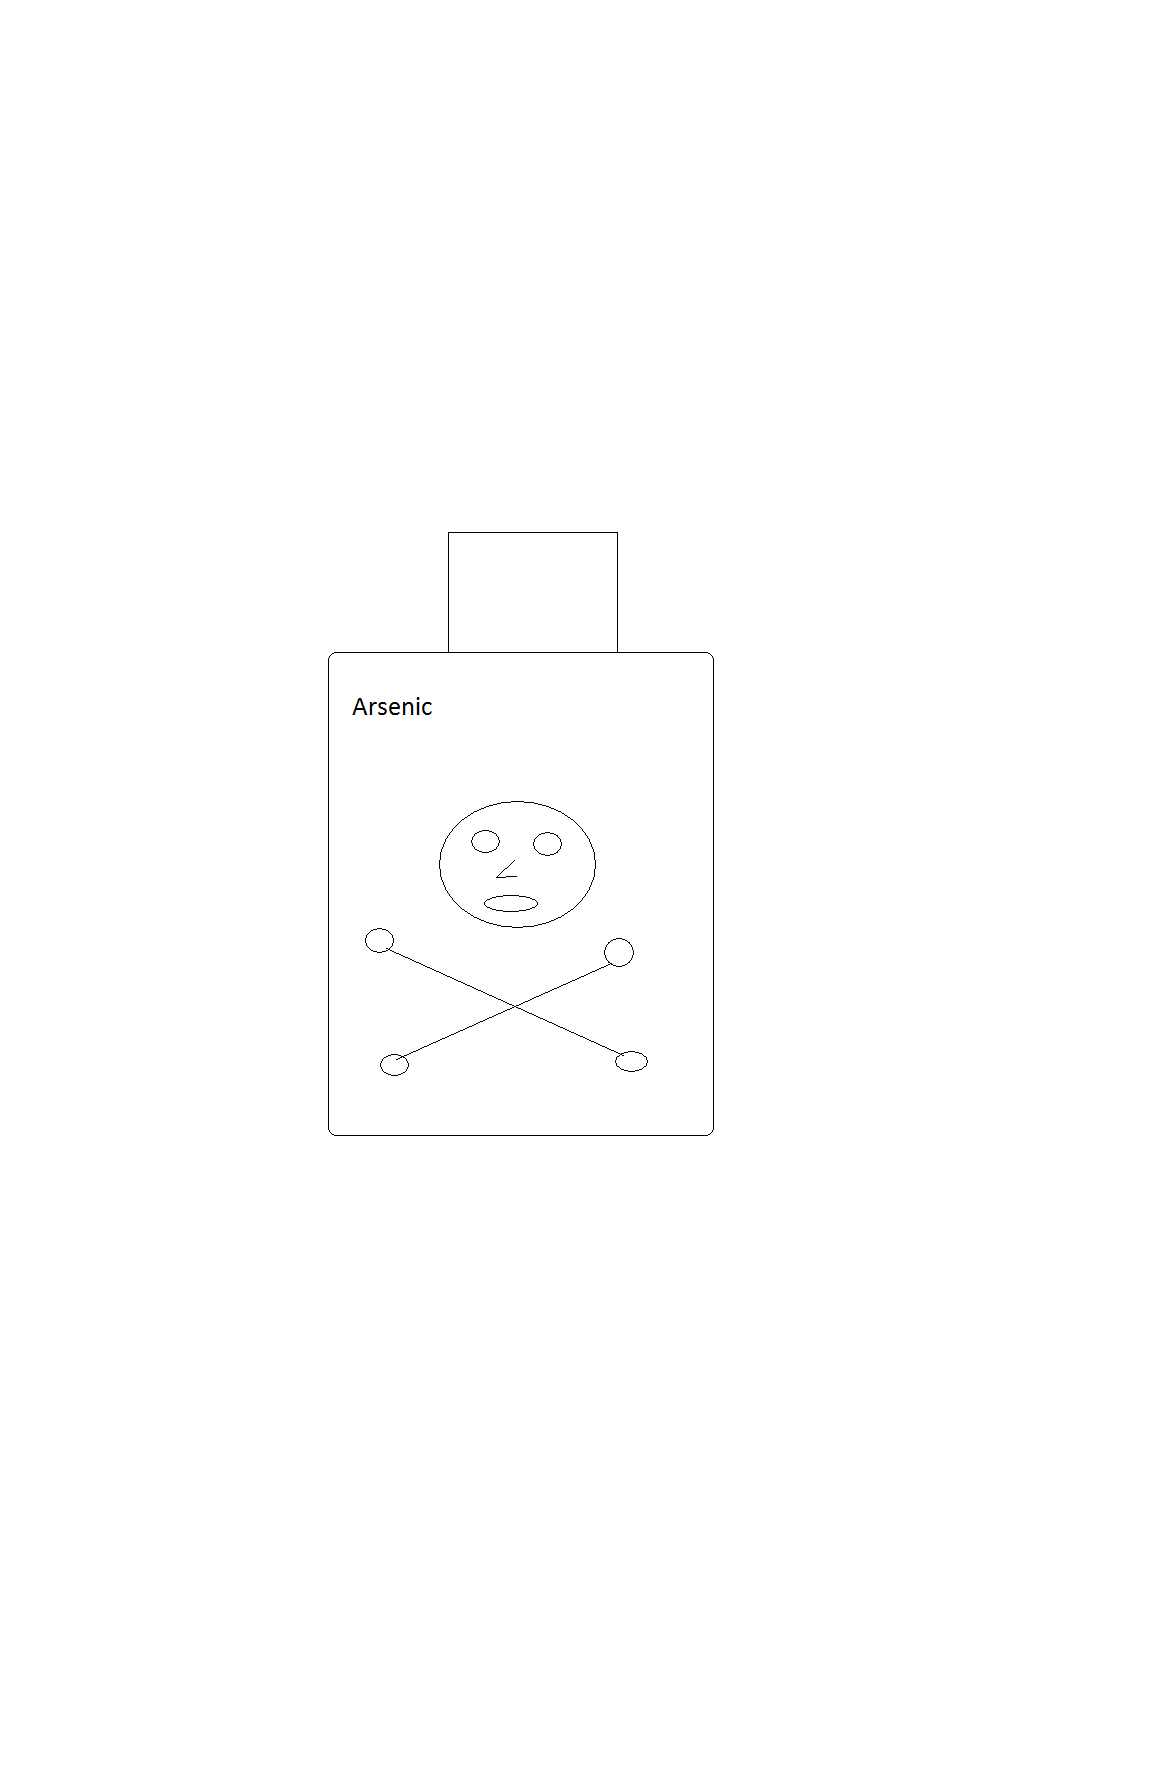
\includegraphics[width=\textwidth]{art/brylcreem-arsenic.png}
  \caption{Artwork by brylcreem}
\end{figure}
